\documentclass[12pt]{article}
\usepackage{amsmath}
\usepackage{amssymb}
\usepackage{geometry}
\usepackage{enumerate}
\usepackage{natbib}
\usepackage{float}%稳定图片位置
\usepackage{graphicx}%画图
\usepackage[english]{babel}
\usepackage{a4wide}
\usepackage{indentfirst}%缩进
\usepackage{enumerate}%加序号
\usepackage{multirow}%合并行
\title{\large UM-SJTU JOINT INSTITUTE\\Intro to Circuits\\(VE215)\\\ \\\ \\\ \\\ \\\ \\\ \\\ \\\ \\\ \\\ \\\
LABORATORY REPORT\\\ \\\ EXERCISE 1\\\  DC Lab \\\ \\\ \\\ \\\ \\\ }
\author{Name: Pan Chongdan\\ID: 516370910121\\Group: 16}
\date{Date: \today}
\begin{document}
\maketitle
\newpage
\section{Objectives}
\begin{enumerate}
\item Learn how to use UT60A multimeter for measurements of voltage, current, and resistance.
\item Learn to build circuits on a solderless prototype board.
\item Verify the basic circuit laws KCL, KVL, and Ohm’s laws from measurements of currents and voltages. 
\item Measure the current-voltage characteristics of a 50$\Omega$ resistor. From the results of measurements, draw the conclusion on whether they obey Ohm’s law.
\item Build an LED circuit on a protoboard and learn about non-ohmic circuit components, which do not obey Ohm’s law.
\end{enumerate}
\section{Apparatus}
\subsection{Multimeter}
A multimeter is able to work as a voltmeter to measure voltages, as an ammeter to measure currents, or as an ohmmeter to measure resistances.
\par Every multimeter has two terminals for the two cables that ensure electrical connections to the two nodes. The black cable should be connected to ground, the ground port is labeled COM on the multimeter. The red cable should be connected to HzV$\Omega$ port for voltage or resistance measurements, 10A MAX port for current measurements, or $\mu$AmA port for small current measurements.
\subsubsection{Voltage Measurement}
The voltmeter has its own internal resistance, which is usually very high. For an ideal voltmeter the input resistance is infinitely large. In real instruments the internal resistance usually exceeds 1M$\Omega$. When we measure $V_{AB}$ the voltmeter’s internal resistance is connected in parallel with all circuit elements between these two terminals. Note that you do not have to change anything in your circuit to measure voltage: just connect the multimeter to the nodes of interest
\subsubsection{Current Measurements}
To measure the current that flows through a branch of your circuit we should make this current flow through the multimeter. Note that in order to measure the current we have to interrupt the circuit.The circuits is broken at the point where we measure the current and the ammeter bridges the gap. The internal resistance of an ammeter is very low, say, 1$\Omega$ or less.
\subsubsection{Resistance Measurements}
First,disconnect the resistance from original circuit.Second, we simply connect it to the two terminals of the multimeter, and read the resistance from the display.
\subsection{DC Source}
\subsubsection{MOTECH LPS 305 Power Supply$^2$}
\begin{figure}[H]
\centering
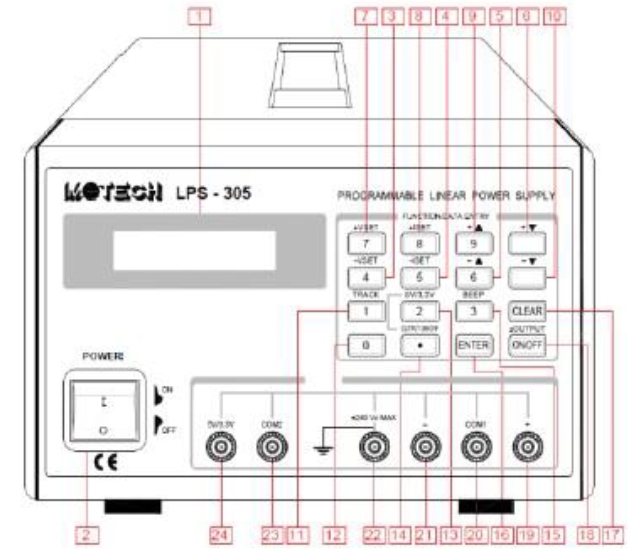
\includegraphics[scale=0.5]{P1.jpg}
\end{figure}
\begin{enumerate}
\item When you press the +Vset, or -Vset, the output selected (+output or –output) and the present setting for that function will be displayed. You can change setting using the numeric entry keys. Pressing the number keys will cause the present numeric setting to become blank and be replaced with the new numbers on the display. Pressing the ENTER key will enter the values displayed.
\item The selected output channel can be turned on and off from the front panel. The output on/off key toggles both the +output and –output on and off simultaneously.
\item Remember to turn off the output when no measurements are being undertaken.
\end{enumerate}
\subsubsection{Agilent E3631A DC Power Supply$^3$}
\begin{figure}[H]
\centering
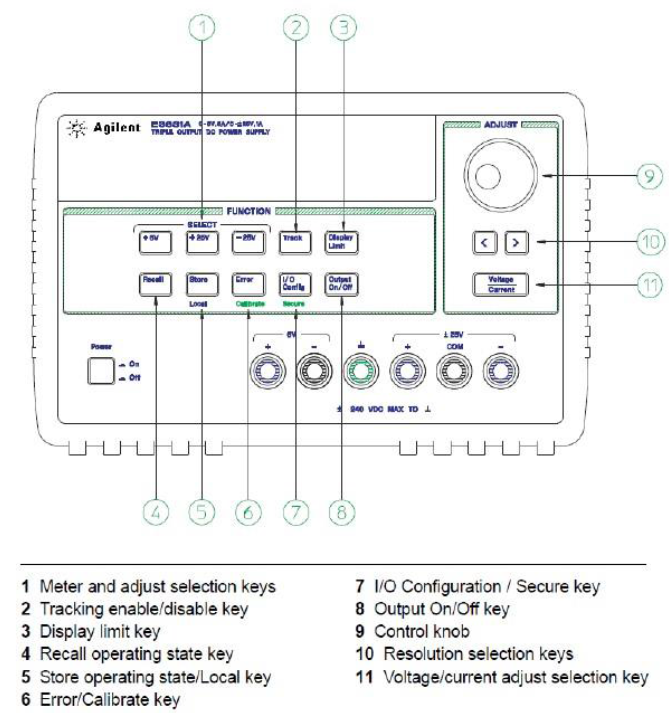
\includegraphics[scale=0.5]{P2.jpg}
\end{figure}
\begin{enumerate}
\item Connect a load to the desired output terminals with power-off.
\item Press to turn on the power supply. The power supply will go into the power-on / reset state; all outputs are disabled (the OFF annunciator turns on); the display is selected for the +6V supply (the +6V annunciator turns on); and the knob is selected for voltage control.
\item Adjust the knob for the desired output voltage. Set the knob for voltage control. The second digit of the voltmeter will be blinking. Adjust the knob to the desired output voltage.
\end{enumerate}
\subsection{Protoboards}
In this lab and all the future labs, you will connect resistors, LEDs and other components to each other on a circuit board. Circuits boards are also called “protoboards”, because they are used for prototyping the circuits. Another name is “breadboard”, because in old times circuits were indeed built on wooden breadboards. The main idea is to build the citcuit without soldering every connection thus the long generic name is solderless prototyping boards.
\par A prototyping board used in the lab consists of several plastic blocks. These plastic blocks are mounted on a metal plate along with terminal (blind) posts.
\par Each plastic block has many holes, into which you insert wires, plug in resistors, op amps, and other circuit components. Inside the plastic block, themetal clips snugly hold your wires, resistors, etc., and ensure electric connections between circuit components.
\begin{figure}[H]
\centering
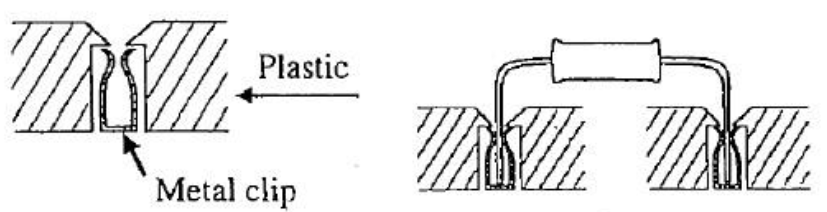
\includegraphics[scale=0.5]{P3.jpg}
\end{figure}
\par These metal clips hidden under the plastic create nodes on the protoboard, to which you connect your circuit components.
\begin{figure}[H]
\centering
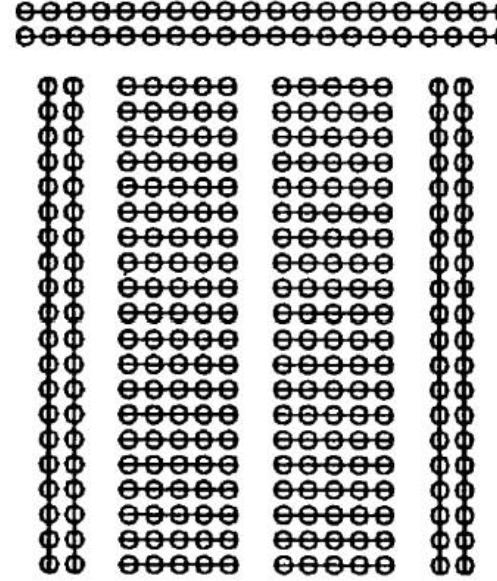
\includegraphics[scale=0.5]{P4.jpg}
\caption{Connections under the plastic}
\end{figure}
\par Straight lines on the diagram above show the metal clips that connect holes under the plastic.Remember how the holes are connected into nodes on a circuit board. Many students’ mistakes in the lab are due to forgetfulness of how the nodes are organized.
\subsection{Semiconductor diodes}
The simplest semiconductor device is a diode. Its circuit symbol looks like an arrow because the diode allows the current flow only in the direction of that arrow. If $V_A>V_B$, the conductor will conduct. If $V_B>V_A$ the conductor will not conduct. Thus a diode is not an Ohmic resistor.
\begin{figure}[H]
\centering
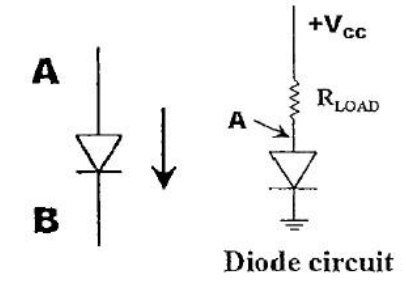
\includegraphics[scale=0.5]{P5.jpg}
\end{figure}
\par Moreover, even under direct bias the resistance of a diode does not remain constant. At small values of the voltage difference $V_A-V_B$ the current through the diode is very small, because itsresistance is large. The diode’s resistance abruptly changes as soon as the direct bias voltage across the diode reaches the threshold value, which is called the turn-on voltage and equals about
0.5 to 0.7V for many diodes. Above this voltage the current through the diode rapidly increases and becomes practically independent of the voltage. The diode resistance becomes so small that in real circuits the diodes have to be protected from high currents that may damage them. A load resistor (50$\Omega$ in this lab) connected in series with the diode ensures the simplest protection.
Light-emitting diodes emit light (visible or infrared) when the direct current becomes large enough. The LED, which you will use in this lab, has the turn-on voltage of about 1.6V.
\section{Results}
\subsection{Voltage,Current \& Resistance Measurement}
\begin{table}[H]
\centering
\begin{tabular}{|c|c|c|c|}
\hline
Resistance{[}$\Omega${]}  & \multicolumn{3}{c|}{100.0}        \\ \hline
Voltage(m){[}V{]} & 2.994 & Voltage(s){[}V{]} & 3.000 \\ \hline
Current(m){[}A{]} & 0.029 & Current(s){[}A{]} & 0.032 \\ \hline
\end{tabular}
\caption{Measurement of voltage, current, and resistance.}
\end{table}
\subsection{Voltage Division \& Current Division}
% Please add the following required packages to your document preamble:
% \usepackage{multirow}
% Please add the following required packages to your document preamble:
% \usepackage{multirow}
\begin{table}[H]
\centering
\begin{tabular}{|c|c|c|c|c|}
\hline
\multirow{3}{*}{} & Resistance R1[$\Omega$]      & 100.0          & Resistance R2[$\Omega$]      & 50.9           \\ \cline{2-5} 
                  & \multicolumn{2}{c|}{Voltage Division} & \multicolumn{2}{c|}{Current Division} \\ \cline{2-5} 
                  & Current[A]           & Voltage[V]     & Current[A]           & Voltage[V]     \\ \hline
Total             & 0.019                & 2.984          & 0.088                & 2.984          \\ \hline
R1                & 0.019                & 1.979          & 0.029                & 2.982          \\ \hline
R2                & 0.019                & 1.009          & 0.058                & 2.980          \\ \hline
\end{tabular}
\caption{Voltage division and current division}
\end{table}
\begin{table}[H]
\centering
\begin{tabular}{|c|c|c|c|c|}
\hline
\multirow{3}{*}{} & Resistance R1[$\Omega$]      & 100.0          & Resistance R2[$\Omega$]      & 50.9           \\ \cline{2-5} 
                  & \multicolumn{2}{c|}{Voltage Division} & \multicolumn{2}{c|}{Current Division} \\ \cline{2-5} 
                  & Current[A]           & Voltage[V]     & Current[A]           & Voltage[V]     \\ \hline
Total             & 0.020               & 3.000          & 0.089                & 3.000          \\ \hline
R1                & 0.020                & 1.988          & 0.030                & 3.000         \\ \hline
R2                & 0.020                & 1.012          & 0.059                & 3.000 \\ \hline
\end{tabular}
\caption{Theoretical voltage division and current division}
\end{table}
\subsection{Ohm's Law}
\begin{table}[H]
\centering
\begin{tabular}{|c|c|c|}
\hline
Resistance[$\Omega$] & 50.9       \\ \hline
Voltage[V]   & Current[A]&Theoretical Current [A] \\ \hline
0.5          & 0.009      &0.010\\ \hline
1.0          & 0.019      &0.020\\ \hline
1.5          & 0.029      &0.029\\ \hline
2.0          & 0.039      &0.039\\ \hline
3.0          & 0.058      &0.059\\ \hline
4.0          & 0.078      &0.079\\ \hline
5.0          & 0.098      &0.098\\ \hline
\end{tabular}
\caption{Ohm's Law}
\end{table}
\begin{figure}[H]
\centering
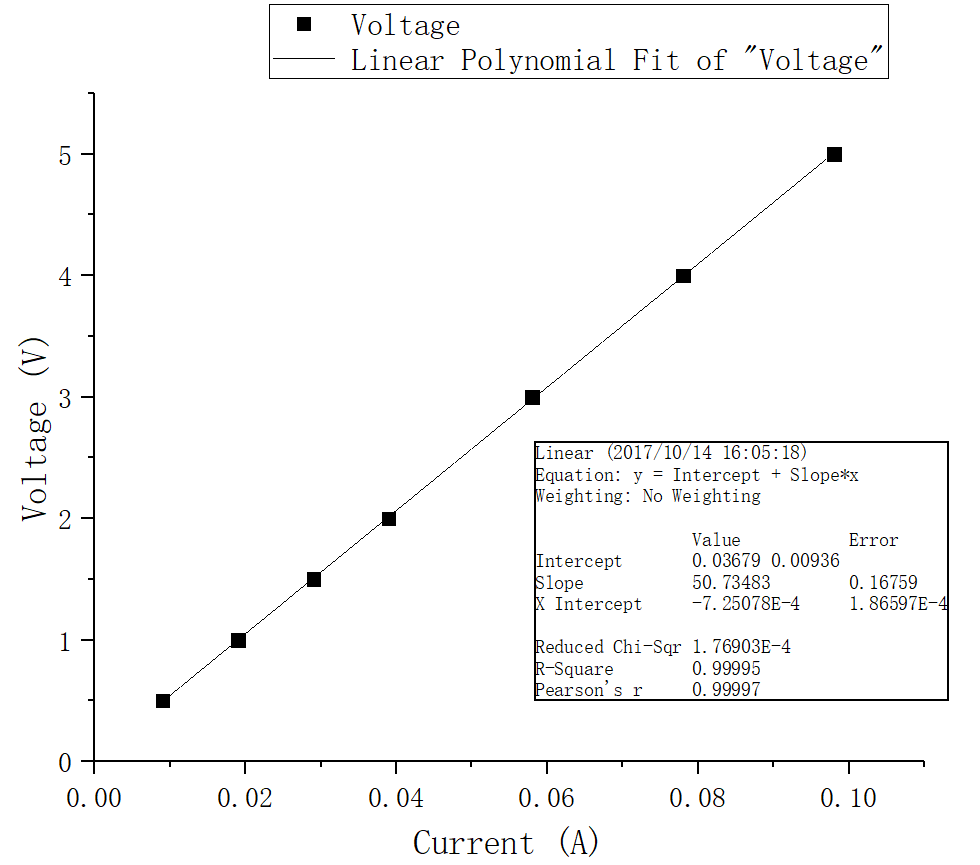
\includegraphics[scale=0.3]{P6.jpg}
\end{figure}
\subsection{Non-ohmic LED}
\begin{table}[H]
\centering
\begin{tabular}{|c|c|c|}
\hline
Source Voltage[V] &Voltage[V]& Current[A] \\ \hline
2.0        &2& 0          \\ \hline
2.5        &2.5& 0          \\ \hline
3.0        &2.85& 0.003      \\ \hline
3.5        &3.05& 0.009      \\ \hline
4.0        &3.4& 0.012      \\ \hline
4.5        &3.3& 0.024      \\ \hline
5.0        &3.4& 0.032      \\ \hline
6.0        &3.55& 0.049      \\ \hline
\end{tabular}
\caption{Semiconductor diodes}
\end{table}
\begin{figure}[H]
\centering
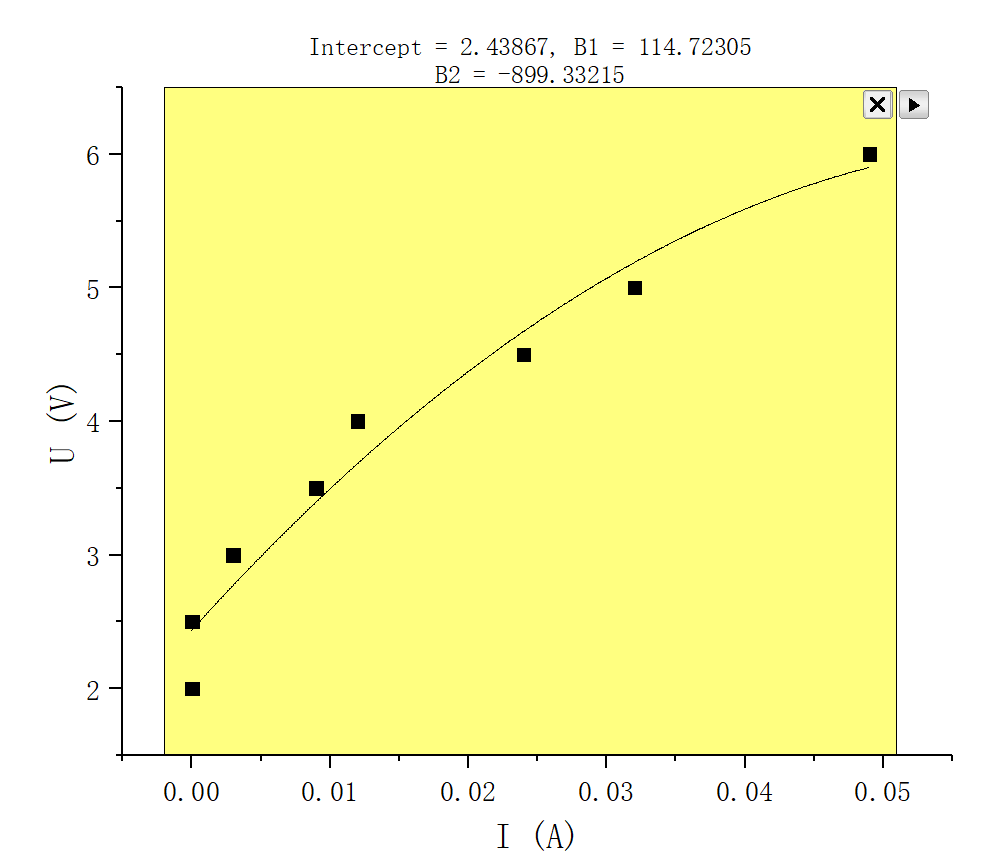
\includegraphics[scale=0.45]{P7.jpg}
\end{figure}
\section{Discussion}
\subsection{Voltage, Current \& Resistance Measurement}
When I measure the resistance, I should disconnect the resistor from the circuit because the power source from the multimeter will provide the voltage. Otherwise, the measured resistance will be incorrect.
\par The measured voltage and current are both less than the theoretical data, I think it's because the wire has resistance which can't be ignored.
\subsection{Voltage Division \& Current Division}
\par The measured voltage and current are also less than the theoretical data, I think it's the same reason above.
\par When the two resistors are connected in series, according to my data in voltage division,the resistors' current are same and the bigger resistance the resistor has, the higher  voltage it has.$$\frac{V_1}{V_2}=\frac{R_1}{R_2}$$
\par When the two resistors are connected in parallel, according to my data in current division,the resistors' voltages are same and the bigger resistance the resistor has, the smaller current it has.$$\frac{I_2}{I_1}=\frac{R_1}{R_2}$$ 
\subsection{Ohm's Law}
From my data, the measured current is less than the theoretical, it's also due to the little resistance caused by the wire. In my linear-fit figure ,the current is in direction proportion to the voltage and the slope is the resistance.
\subsection{Non-ohmic Led}
Even though the semiconductor is non-ohmic, its current will still be bigger as long as the voltage is bigger but it isn't in direction proportion to the voltage any more. The semiconductor's resistance will be smaller first, and then it will be bigger with the increase of the voltage.
\par In my table of this measurement, when the voltage between the Led is equal to 3.4V, it has two different current, I think I must have made some mistake in it. 
\par In addition, as the Voltage becomes bigger, the slope of the figure also become smaller, which means the resistance of the LED is becoming lower, which agrees with its characteristic.
\section{Conclusion}
In this lab, I review the usage of multimeter and learn how to use DC source and a protoboard to build a circuit. In addition, I build my own circuit to prove the Ohm's Law, current division  principle, and voltage division principle. Moreover, I examine the voltage-current character of semiconductor diode, which is a non-omhic Led.
\section{Reference}
\begin{enumerate}[-]
\item \emph{VE215FA2017 DCLabManual} 
\item \emph{Circuits Make Sense}, Alexander Ganago, Department of Electrical Engineering and Computer Science, University of Michigan, Ann Arbor.
\end{enumerate}
\end{document}